
\chapter{Sparse grids combination technique}



% TD:
% add info about mixed regularity assumption


Introduced in 1963 by Russian mathematician Smolyak\cite{smolyak}, the sparse grid method
is a discretization technique for handling problems of high dimensionality.
It was first introduced for the integration of multidimensional functions,
but it has since found a broader range of applications, including in
numerical methods for solving partial differential equations.

In the discretization of PDEs, we usually construct
simple uniform grids which contain on the order $O(N^d)$ degrees of freedom,
where $d$ is the spatial dimension of the problem and $N$
denotes the number of grid points in a single spatial dimension.
The discretization performed in sparse grids, on the other hand,
leads to only $O(N(\log{N})^{d-1})$ degrees of freedom.\cite{sg_123}

In addition, provided that the problem is smooth enough, 
the accuracy obtained in this way is comparable to the full-grid approach.

This makes the sparse-grid construction particularly attractive for
moderate to high dimensional problems.
%Still due to the logarihgm term, the curse of dimensiinality is still present.
%Buts if effect is weakened.
%Herem, the grids requited involves only $O(n(\log(n)^{d-1}))$
%the curse of dim can be overcame to some extend by some extend by the sparse grid construction.
%THe discreatizaiton performed in sparse grids involves only $O(n(\log(n)^{d-1}))$
%Compared to the $O(n^d)$ requited for full grid approach. 
In the context of PDEs, the so-called \emph{combination technique} has been developed.\cite{combitech}
The combination technique approximates the full grid by a collection of anisotropic grids,
on which the linear algebraic system
arising from the discretization of the PDE can be solved independently.
This decomposition can be strongly exploited on modern parallel computational
architectures. \cite{combitech}
It is this branch of the sparse grids method that we consider in this thesis.

The following sections first give a brief introduction to the sparse-grid method and
to the combination technique.
The final sections describe the implementation of the method.
%are given in the last section of this chapter.
%For the educational purposes of this thesis, the combination technique has been
%implemented from scratch.



\subsection{1-dimensional hierarchical basis}

In the classical sparse-grid approach,
the basis is built from the standard linear hat functions

$$
\phi(x)=
\begin{cases}
1-|x|, & |x|\le 1,\\
0, & |x|>1.
\end{cases}
$$

Consider a set of equidistant grids $\Omega_l$ of level $l\in\mathbb{N}$ on the one-dimensional unit interval $\bar{\Omega}=\left[0,1\right]$

$$
\Omega_l := \{x_{l,i}=i\cdot h_l : 0\le i\le 2^l\}
$$

For each level $l$, we define the mesh width $h_l$ as
$$
h_l := 2^{-l}
$$

The standard hat function $\phi$ is then used to generate a set of basis functions $\phi_{l,i}$
with support $\left[ x_{l,i}-h_l, x_{l,i}+h_l \right]$


$$
\phi_{l,i}(x)
=
\phi\!\left(\frac{x-x_{l,i}}{h_l}\right),
\qquad 1\le i\le 2^l-1.
$$

These basis functions are then used to define the finite element space $V_l$ as
$$
V_l := \mathrm{span}\{\phi_{l,i} : 1\le i\le 2^l-1\}
$$

Next, we decompose this space into hierarchical increments by constructing the so-called
\textit{hierarchical increment spaces} $W_l$, as
\begin{gather*}
W_l := \mathrm{span}\{\phi_{l,i}: i\in I_l\}\,,\\
I_l := \{\, i\in\mathbb{N} : 1\le i\le 2^l-1,\ i\ \text{odd}\,\}
\end{gather*}
where $I_l$ are the hierarchical index sets.

A visual representation of the definitions given so far is provided in the figure below:

\vspace{1em}
\begin{center}
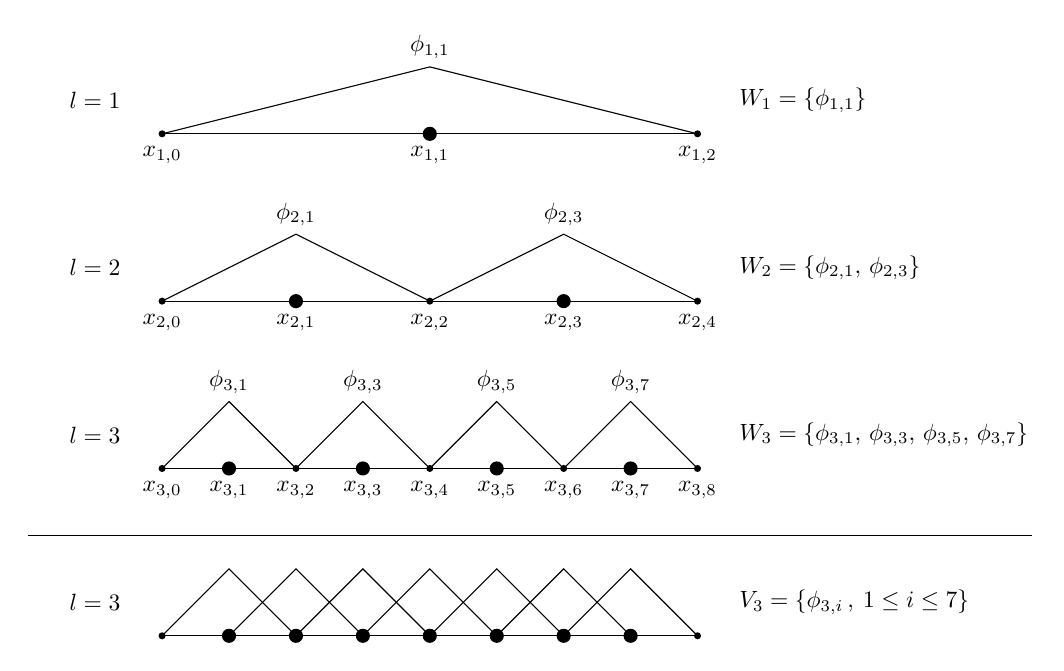
\begin{tikzpicture}[xscale=0.85, yscale=0.85, transform shape]

    % Level 1
    \def\y{7.5}
    \node[left] at (-0.5, \y+0.5) {$l=1$};
    \node[right] at (8.5, \y+0.5) {$W_1=\{\phi_{1,1}\}$};
    %\node[left] at (10, \y) {$\Omega_1=\{x_{1,0}, x_{1,1}, x_{1,2}\}$};
    %\node[left] at (10, \y+0.5) {$I_1=\{1\}$};
    %\node[left] at (10, \y+1.5) {$W_1=\{\phi_{1,1}\}$};
    \draw (0,\y) -- (8,\y); % Domain line
    \draw (0,\y) -- (4,\y+1) -- (8,\y); % Basis function
    \node[above] at (4,\y+1) {$\phi_{1,1}$};
    
    % Grid points for l=1
    \fill (0,\y) circle (1.5pt) node[below, yshift=-2pt] {$x_{1,0}$};
    \fill (4,\y) circle (3pt)   node[below, yshift=-2pt] {$x_{1,1}$}; % Larger/bolder point
    \fill (8,\y) circle (1.5pt) node[below, yshift=-2pt] {$x_{1,2}$};

    % Level 2
    \def\y{5.0}
    \node[left] at (-0.5, \y+0.5) {$l=2$};
    \node[right] at (8.5, \y+0.5) {$W_2=\{\phi_{2,1},\,\phi_{2,3}\}$};
    \draw (0,\y) -- (8,\y);
    \draw (0,\y) -- (2,\y+1) -- (4,\y);
    \draw (4,\y) -- (6,\y+1) -- (8,\y);
    \node[above] at (2,\y+1) {$\phi_{2,1}$};
    \node[above] at (6,\y+1) {$\phi_{2,3}$};
    
    % Grid points for l=2
    \foreach \i in {0,2,4} {
        \pgfmathsetmacro{\x}{\i*2}
        \fill (\x,\y) circle (1.5pt) node[below, yshift=-2pt] {$x_{2,\i}$};
    }
    \foreach \i in {1,3} {
        \pgfmathsetmacro{\x}{\i*2}
        \fill (\x,\y) circle (3pt) node[below, yshift=-2pt] {$x_{2,\i}$}; % Bolder points
    }

    % Level 3
    \def\y{2.5}
    \node[left] at (-0.5, \y+0.5) {$l=3$};
    \node[right] at (8.5, \y+0.5) {$W_3=\{\phi_{3,1},\,\phi_{3,3},\,\phi_{3,5},\,\phi_{3,7}\}$};
    \draw (0,\y) -- (8,\y);
    
    % Basis functions and active points for l=3
    \foreach \i in {1,3,5,7} {
        \draw (\i-1,\y) -- (\i,\y+1) -- (\i+1,\y);
        \node[above] at (\i,\y+1) {$\phi_{3,\i}$};
        \fill (\i,\y) circle (3pt) node[below, yshift=-2pt] {$x_{3,\i}$};
    }
    % Inactive points for l=3
    \foreach \i in {0,2,4,6,8} {
        \fill (\i,\y) circle (1.5pt) node[below, yshift=-2pt] {$x_{3,\i}$};
    }

    \def\y{1.5}
    \draw (-2,\y) -- (13,\y);

    % Level 3 for V_3
    \def\y{0.0}
    \node[left] at (-0.5, \y+0.5) {$l=3$};
    %\node[right] at (8.5, \y+0.5) {$V_3=\{\phi_{3,1},\,\phi_{3,2},\,\phi_{3,3},\,\phi_{3,4},\,\phi_{3,5},\,\phi_{3,6}$\}};
    \node[right] at (8.5, \y+0.5) {$V_3=\{\phi_{3,i}\,,\: 1\le i \le 7\}$};
    \draw (0,\y) -- (8,\y);

    \foreach \i in {1,2,3,4,5,6,7} {
        \draw (\i-1,\y) -- (\i,\y+1) -- (\i+1,\y);
        %\node[above] at (\i,\y+1) {$\phi_{3,\i}$};
        \fill (\i,\y) circle (3pt); %node[below, yshift=-2pt] {$x_{3,\i}$};
    }
    \foreach \i in {0,8} {
        \fill (\i,\y) circle (1.5pt); %node[below, yshift=-2pt] {$x_{3,\i}$};
    }


\end{tikzpicture}
\end{center}
\vspace{1em}


The decomposition of $V_l$ is then given by the direct-sum formula
$$
V_l = \bigoplus_{k=1}^l W_k
$$


Every function $u\in V_l$ can then be represented uniquely as
$$
u(x)=\sum_{k=1}^l \sum_{i\in I_k} v_{k,i}\,\phi_{k,i}(x),
$$
where $v_{k,i}\in \mathbb R$ are called \textit{hierarchical surpluses}.
An important feature of this decomposition is that all basis functions $\phi_{k,i}$
spanning the same space $W_k$ have mutually disjoint support (see again the figure above).


\subsection{Tensor product construction in higher dimensions}


Next, we move to a $d$-dimensional unit cube $\bar{\Omega}=\left[0,1\right]^d$.
We discretize this space by a collection of grids, where
each grid is equidistant with respect to each individual coordinate direction,
but, in general, has varying mesh sizes in those different directions. 
The construction is analogous to the one-dimensional case presented above.
%where the the hierarchical basis in obtained as a tensor product of the indivisual 1-dimensional bases.

Let $\mathbf{l}=(l_1,\dots,l_d)\in\mathbb{N}^d$ be a multi-index of levels.
We then define the mesh spacing at the individual levels $h_\mathbf{l}\in\mathbb{R}^d$
and a grid point $x_{\mathbf{l},\mathbf{i}}\in\mathbb{R}^d$
$$
h_\mathbf{l} :=  2^{-\mathbf{l}} = (2^{-l_1},\dots,2^{-l_d}),
$$
$$
x_{\mathbf{l},\mathbf{i}}
%:= (x_{l_1,i_1},\dots,x_{l_d,i_d})
:= (i_1\,2^{-l_1},\dots,i_d\,2^{-l_d})\,,\quad
\mathbf{i}=(i_1,\dots,i_d)\in\mathbb{N}^d
$$
The collection of such points on level $\mathbf l$ then forms a grid $\Omega_\mathbf{l}$.

The tensor-product basis functions are then defined as a product of one-dimensional hat functions
$$
\phi_{\mathbf{l},\mathbf{i}}(\mathbf{x})
=
\prod_{j=1}^d \phi_{l_j,i_j}(x_j),
\qquad \mathbf{x}=(x_1,\dots,x_d)
$$

The corresponding tensor-product finite element space is then
$$
V_\mathbf{l} := \mathrm{span}\{\phi_{\mathbf{l},\mathbf{i}}: 1\le \mathbf{i} \le 2^\mathbf{l}-1\},
$$
and the hierarchical increment space is
$$
W_\mathbf{l} := \mathrm{span}\{\phi_{\mathbf{l},\mathbf{i}}: \mathbf{i}\in I_\mathbf{l}\},
$$
$$
I_\mathbf{l}
=
\left\{
i\in\mathbb{N}^d:\ 1\le \mathbf{i} \le 2^\mathbf{l}-1,\ \text{and each } i_j \text{ is odd}
\right\}.
$$

Again,
$$
V_\mathbf{l} = \bigoplus_{\mathbf{k}\le \mathbf{l}} W_\mathbf{k},
$$
where the inequality sign $\le$ is interpreted componentwise.

Next, the support of any two hierarchical basis functions $\phi_{\mathbf{l}, \mathbf{k}}$
spanning the same space $W_\mathbf{l}$ is disjoint.

And also, each function $u\in V_\mathbf{l}$ admits a unique representation
$$
u(\mathbf{x})
=
\sum_{\mathbf{k}\le \mathbf{l}} \sum_{\mathbf{i}\in I_\mathbf{k}}
v_{
    \mathbf{k},
    \mathbf{i}
}\,\phi_{
    \mathbf{k},
    \mathbf{i}
}(\mathbf{x})
$$
with hierarchical coefficients $v_{\mathbf{k},\mathbf{i}}\in\mathbb{R}$.


\subsection{From full grids to sparse grids}

If one fixes a maximal one-dimensional level $n$ in each coordinate, one obtains the classical full tensor-product space
$$
V_n := V_{(n,\dots, n)}
=
\bigoplus_{|\mathbf l|_\infty\le n} W_\mathbf{l}.
$$
Its dimension behaves like
$$
\dim V_n = O(2^{nd}).
$$
This is the usual curse of dimensionality.

To improve this, we formulate the following cost-benefit argument in
function approximation:
we seek a finite collection of subspaces $W_\mathbf{l}$ that
maximize the approximation benefit of adding that space, against a cost
coming from the introduced degrees of freedom.

%Under the conditoin of mixed regularity, that the approximation lives in the following space
%$$
%H_2^{mix}(\overline\Omega) = \{u : \overline{\Omega} \rightarrow \mathbb{R} :
%D^\alpha u \in L_2(\Omega), |\alpha|_\infty \le 2,\:\:
%u|_{\partial\Omega} = 0
%\}
%$$
%$$
%D^\alpha u := \frac{ \partial^{|\mathbf{\alpha}|_1} u }{ \partial x_1^{\alpha_1} \cdots \partial x_d^{\alpha_d} }
%$$
%
%$$
%|\alpha|_1 = \sum^d_{j=1} \alpha_j, \quad |\alpha|_\infty = \max_{1\le i\le d} \alpha_j
%$$

%The local cost of including a subspace $W_l$ is its dimension (the number of degrees of freedom):
%\begin{equation}
%c(l) := |W_l| = 2^{|l|_1-d}
%\end{equation}
%
%The local benefit is bounded by the squared norm of the contribution $u_l$.
%
%For this purpose, let us define the space of functions with bounded mixed derivatives:
%We then consider the space of functions with bounded mixed derivatives:
%
%$$
%X^{q,r}(\overline{\Omega}) := \{u : \overline{\Omega} \rightarrow \mathbb{R} : D^\alpha u \in L_q(\Omega), |\alpha|_\infty \le r \}
%$$
%$$
%X_0^{q,r}(\overline{\Omega}) := \{u \in X^{q,r}(\overline{\Omega}): u|_{\partial\Omega} = 0\}
%$$
%Under the bounded mixed derivatives assumption ($|u|_{2,\infty} < \infty$), the bounds decay rapidly.
%Specifically, $||u_l||_\infty \le 2^{-d} 2^{-2|l|_1} |u|_{2,\infty}$.
%Defining the cost-benefit ratio $cbr(l) = b(l)/c(l)$,
%an optimal grid contains all subspaces $W_l$ where the cost-benefit ratio is above a certain threshold.
%\begin{equation}
%|l|_1 \le n + d - 1
%\end{equation}
%This explicitly defines the standard sparse grid space $V_n^{(1)}$:
%\begin{equation}
%V_n^{(1)} := \bigoplus_{|l|_1 \le n + d - 1} W_l
%\end{equation}
%which is Linf and L2-optimal with respect to our cost-benefit setting

Under the assumption of mixed regularity of the approximation, the sparse-grid construction keeps only the subspaces satisfying
$$
|\mathbf{l}|_1 \le n+d-1.
$$

This leads to the definition of the \emph{sparse-grid} space $\widehat V_n$ of level $n$,
$$
\widehat V_n
:=
\bigoplus_{|\mathbf l|_1\le n+d-1} W_\mathbf{l}.
$$

The number of degrees of freedom (the number of grid points) is then only
$$
\dim \widehat V_n
=
\sum_{i=0}^{n-1} 2^i \binom{d-1+i}{d-1}
= O(h_n^{-1}|\log_2(h_n)|^{d-1})
= O(2^n n^{d-1}).
$$
where $h_n=2^{-n}$.
Note that for $N=2^n$ this gives the stated $O(N(\log{N})^{d-1})$ dependence.

On the other hand, for functions satisfying the regularity conditions,
the interpolation error of the sparse-grid approximation $\widehat u_n\in\widehat V_n$ satisfies
$$
\|u-\widehat u_n\|_{L^2(\Omega)}
=
O(h_n^2\:n^{d-1}),
\qquad
\|u-\widehat u_n\|_{L^\infty(\Omega)}
=
O(h_n^2\:n^{d-1}).
$$
Thus, compared with the full-grid error $O(h_n^2)$, the error is scaled approximately polynomially with dimension.
\cite{sg_123}

The following table summarizes the main differences between the full-grid and sparse-grid constructions:

\renewcommand{\arraystretch}{1.5}
\begin{center}
\begin{tabular}{c c c}
    \hline
    \textbf{grid space} & \textbf{degrees of freedom} & \textbf{$L^2$ and $L^\infty$ error} \\
    \hline
    $V_n=\bigoplus_{|\mathbf l|_\infty\le n} W_\mathbf{l}$ & $\dim(V_n)=O(2^{nd})$ & $\|u-u_n\|_{L^p(\Omega)}=O(h_n^2)$ \\
    $\widehat V_n=\bigoplus_{|\mathbf l|_1\le n+d-1} W_\mathbf{l}$ & $\dim(\widehat V_n)=O(2^n n^{d-1})$ & $\|u-\widehat u_n\|_{L^p(\Omega)}=O(h_n^2\:n^{d-1})$ \\
\end{tabular}
\end{center}
\vspace{1em}



\subsection{Combination technique}

For the numerical solution of partial differential equations,
the so-called \emph{combination technique} is commonly employed.

In this method, the approximation $\widehat u_n$ is given as a
weighted combination of solutions on the anisotropic
grids $\Omega_\mathbf{l}$
based on the combination formula

$$
\widehat u_n(\mathbf x)
=
\sum_{n\le |\mathbf l|_1\le n+d-1}
(-1)^{n+d-1-|\mathbf l|_1}
\binom{d-1}{|\mathbf l|_1-n}
u_\mathbf{l}(\mathbf x)
$$

where $u_\mathbf{l}$ is a solution on the anisotropic grid
$\Omega_\mathbf{l}$ of mesh size $2^{-\mathbf l}$.

%Note, that since we require $l_j>1$ for $j=1,\dots,d$,
%then in the case $n<d$ the lower bound on $|\mathbf l|_1$ changes to $d$.

Notice that, in comparison to the construction of $\widehat V_n$,
the levels $\mathbf l$ in the combination formula above are bounded below by $n$.

%So, for the case $d=2$, we get the combination formula
%$$
%\sum_{|\mathbf l|_1=n+1}
%u_\mathbf{l}(\mathbf x)
%-
%\sum_{|\mathbf l|_1=n}
%u_\mathbf{l}(\mathbf x)
%$$
%
%In $d=3$, we get
%$$
%\sum_{|\mathbf l|_1=n+2}
%u_\mathbf{l}(\mathbf x)
%- 2
%\sum_{|\mathbf l|_1=n+1}
%u_\mathbf{l}(\mathbf x)
%+
%\sum_{|\mathbf l|_1=n}
%u_\mathbf{l}(\mathbf x)
%$$


For example, the case $d=2,\:n=3$ gives
$$
|\mathbf l|_1 \in \{3,4\}
$$
hence we get the anisotropic grids
$$
\Omega_{(1,2)},\:\,
\Omega_{(2,1)},\:\,
\Omega_{(1,3)},\:\,
\Omega_{(2,2)},\:\,
\Omega_{(3,1)}
$$
Note that in the context of the combination technique,
such grids are commonly referred to as \emph{component grids}.


%\documentclass{article}
%\usepackage{tikz}
\usetikzlibrary{decorations.pathreplacing}
%\begin{document}

\begin{figure}[htbp]
    \centering
    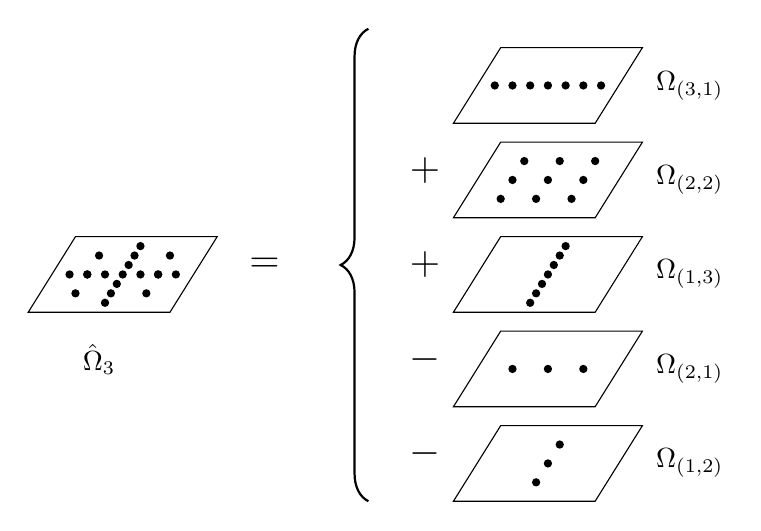
\begin{tikzpicture}[
        scale=1.2,
        % Define the style for the grid points
        point/.style={circle, inner sep=0pt, minimum size=3pt, fill=black}
    ]

    % Define a custom slanted coordinate system to mimic the 3D perspective
    \tikzset{
        slant cs/.style={
            x={(1.5cm,0cm)}, y={(0.5cm,0.8cm)}
        }
    }

    % Command to draw the bounding box for each grid domain
    \newcommand{\gridbox}[2]{
        \begin{scope}[shift={(#1,#2)}, slant cs]
            \draw (0,0) -- (1,0) -- (1,1) -- (0,1) -- cycle;
        \end{scope}
    }

    % --- LEFT SIDE: SPARSE GRID \hat{\Omega}_3 ---
    % Vertically centered relative to the right-side grids
    \gridbox{-1}{2}
    \begin{scope}[shift={(-1,2)}, slant cs]
        % Draw all points that make up the sparse grid
        \foreach \y in {1,2,...,7} { \node[point] at (1/2, \y/8) {}; }
        \foreach \x in {1,3} {
            \foreach \y in {1,2,3} { \node[point] at (\x/4, \y/4) {}; }
        }
        \foreach \x in {1,2,3,5,6,7} { \node[point] at (\x/8, 1/2) {}; }
        
        \node[below=8pt] at (0.5, 0) {$\hat{\Omega}_3$};
    \end{scope}

    % EQUALS SIGN
    \node at (1.5, 2.5) {\Large $=$};

    % LARGE BRACE
    \draw[decorate, decoration={brace, amplitude=10pt}, thick]
        (2.6, 0) -- (2.6, 5);

    % --- RIGHT SIDE: COMBINATION GRIDS ---

    % Grid 1: \Omega_{(3,1)} (|l|_1 = 4)
    \gridbox{3.5}{4}
    \begin{scope}[shift={(3.5,4)}, slant cs]
        \foreach \x in {1,2,...,7} { \node[point] at (\x/8, 1/2) {}; }
        \node[right=10pt] at (1, 0.5) {$\Omega_{(3,1)}$};
    \end{scope}

    % Grid 2: \Omega_{(2,2)} (|l|_1 = 4)
    \node at (3.2, 3.5) {\Large $+$};
    \gridbox{3.5}{3}
    \begin{scope}[shift={(3.5,3)}, slant cs]
        \foreach \x in {1,2,3} {
            \foreach \y in {1,2,3} { \node[point] at (\x/4, \y/4) {}; }
        }
        \node[right=10pt] at (1, 0.5) {$\Omega_{(2,2)}$};
    \end{scope}

    % Grid 3: \Omega_{(1,3)} (|l|_1 = 4)
    \node at (3.2, 2.5) {\Large $+$};
    \gridbox{3.5}{2}
    \begin{scope}[shift={(3.5,2)}, slant cs]
        \foreach \y in {1,2,...,7} { \node[point] at (1/2, \y/8) {}; }
        \node[right=10pt] at (1, 0.5) {$\Omega_{(1,3)}$};
    \end{scope}

    % Grid 4: \Omega_{(2,1)} (|l|_1 = 3)
    \node at (3.2, 1.5) {\Large $-$};
    \gridbox{3.5}{1}
    \begin{scope}[shift={(3.5,1)}, slant cs]
        \foreach \x in {1,2,3} { \node[point] at (\x/4, 1/2) {}; }
        \node[right=10pt] at (1, 0.5) {$\Omega_{(2,1)}$};
    \end{scope}

    % Grid 5: \Omega_{(1,2)} (|l|_1 = 3)
    \node at (3.2, 0.5) {\Large $-$};
    \gridbox{3.5}{0}
    \begin{scope}[shift={(3.5,0)}, slant cs]
        \foreach \y in {1,2,3} { \node[point] at (1/2, \y/4) {}; }
        \node[right=10pt] at (1, 0.5) {$\Omega_{(1,2)}$};
    \end{scope}

    \end{tikzpicture}
    \caption{Combination technique in two dimensions for level $n=3$.} %combining coarse full grids $\Omega_l$, $|l|_1 \in \{3,4\}$.}
\end{figure}
%\end{document}



In general, for a sparse-grid combination technique of level $n$ in dimension $d$,
the number of component grids is:
$$
\binom{n+d-1}{d+1}
$$
which, for fixed $d$, grows polynomially with $n$.
%TD: [show plot : n vs number of componetns grids - for fixed d=2,4,6]


% pg 28 of discoAdapt.pdf - time dep pdes - combining grids at intervals
% pf 41 - CFL condition on time step size - each can at diff rate

%However, in the combination technique, we separete the problem into several subproblems which can be solve independently
%on anisotropic but cheap full grids called \emph{component grids}.
%Such approach offers several benefits.

However, since the solution is obtained as a combination
over independent grids, we can reuse existing full-grid solvers
and solve each grid separately. As a result, each
solver can be run in parallel and the results combined at the end of the computation.
This makes the combination technique computationally very appealing, as it can
leverage the parallel nature of existing hardware.
\cite{discoadapt}

The algorithmic realization of the combination technique is given below:

%\subsection{The sg}
%
%energy norm
%
%o n (log n)d-1
%
%1 d multilevel basis
%
%grid $\Omega_l$ of level l - $2^l$ points
%
%basis function on each grid point with 0 support
%
%space $V_l$
%
%increment spaces $W_l$
%
%$V_l = sum k<l W_k$
%
%hierarchical basis
%
%$u(x) = sum sum v_ik \phi_ik (x) $
%
%
%in high dim:
%
%interval -> rectangles
%
%$phi = \prod_{i=1}^d phis$
%
%---
%classical sg
%
%multiindex of derivatives
%sobol space $u \in L2$, 0 on bc
%
%only combine some rect grids - $\hat{V}_n$
%-> number of dog -> $n (log n)^d-1$
%
%accuracy only slightly(?) worse
%
%--- 
%sg optimized for 
%- energy norm problems
%- sobolev norms
%
%higher order polynomials
%non-smooth problem? - local adaptive refinement
%
%use FEM to discretize, sg to solve
%
%for pdes:
%combination technique
%- optimized for the particular differential operator
%
%
%----------
%
%enegy based norm - no curse
%
%
%
%\section{Most important}
%
%crutial in high dim:
%
%- parallelization
%
%

\begin{algorithm}[H]
\caption{Combination technique}
\begin{algorithmic}[1]
    \Require rectangular domain $\Omega$, time interval $[0,T]$, sparse-grid level $n$, time step $\Delta t$, parameter $\theta \in [0,1]$
    \State Construct the multi-index set
    $$
    \mathcal I_{n,d}
    =
    \left\{
    \mathbf l \in \mathbb N^d : n \le |\mathbf l|_1 \le n+d-1
    \right\}
    $$
    \ForAll{$\mathbf l \in \mathcal I_{n,d}$} \textbf{(in parallel)}
        \State Construct the full anisotropic component grid $\Omega_\mathbf l$
        %\State Project the initial condition onto $\Omega_\mathbf l$
        \State Assemble the discrete spatial differential operator $L_\mathbf l$
        \State Fill $u_\mathbf l^0$ based on the initial condition
        \State Set $N=T / \Delta t$
        \For{$j = 0, \dots, N-1$}
            \State Advance one time step by
            $$
            \left(I-\theta \,\Delta t\, L_\mathbf l\right) u_\mathbf l^{j+1}
            =
            \left(I+(1-\theta)\,\Delta t\, L_\mathbf l\right) u_\mathbf l^j
            $$
            \State where $\theta=0$ gives Euler, $\theta=1$ backward Euler, and $\theta=0.5$ gives the Crank--Nicolson scheme.
        \EndFor
        \State Store the terminal solution $u_\mathbf l(T):=u_\mathbf l^N$
    \EndFor
    \State Interpolate all component solutions to a common grid
    \State Combine the terminal solutions according to the combination formula
    $$
    \widehat u_n(T, \mathbf x)
    =
    \sum_{\mathbf l \in \mathcal I_{n,d}}
    (-1)^{n+d-1-|\mathbf l|_1}
    \binom{d-1}{|\mathbf l|_1-n}
    u_\mathbf{l}(T, \mathbf x)
    $$
    \State \Return $\widehat u_n(T,\mathbf x)$
\end{algorithmic}
\end{algorithm}

Here, each component grid $\Omega_{\mathbf l}$ is treated as an
independent full-grid problem,
and the same spatial discretization and time stepping
scheme is applied on every component grid.

Moreover, the discrete operators have the same tensor-product
structure as in standard finite-difference discretizations. In one spatial
dimension, the second derivative is represented by a tridiagonal matrix
with the Laplace stencil $(1,-2,1)$, while the first derivative is approximated by the
central-difference stencil $(-1,0,1)$. In higher dimensions, these one-dimensional operators
are combined using Kronecker products and thus mapped onto the full tensor grid.

Lastly, since the final solutions $u_\mathbf{l}(T,\mathbf x)$ are defined on different
anisotropic grids, they cannot be trivially summed together. Instead, they are first
evaluated on a common target grid and only then combined via the summation formula.


%For example, for
%$$
%\partial_t u
%=
%a \Delta u + b(\mathbf x)\cdot \nabla u + c(\mathbf x)u,
%$$
%the discrete operator on $\Omega_{\mathbf l}$ takes the form
%$$
%L_{\mathbf l}
%=
%a \sum_{j=1}^d
%\left(
%I \otimes \cdots \otimes D^{(2)}_j \otimes \cdots \otimes I
%\right)
%+
%\sum_{j=1}^d \operatorname{diag}(b_j)\, D^{(1)}_j
%+
%\operatorname{diag}(c),
%$$
%where $D^{(1)}_j$ and $D^{(2)}_j$ denote the lifted first- and second-derivative
%matrices in direction $j$. Thus, in the isotropic diffusion case one recovers
%the familiar five-point type structure in two dimensions, whereas non-diagonal
%diffusion matrices introduce additional mixed-derivative couplings through terms
%of the form $D^{(1)}_i D^{(1)}_j$.

%Note that hte discreatization scheme, iratetive method for hte linear system Ax=b, preditioner, times step
%- are all problem dependet.

\section{Implementation}
We implement the sparse-grid combination technique using the established SG++ sparse-grids toolkit
through its Python bindings.
Some existing combination-technique-specific software exists\cite{discoadapt},
but its setup and adaptation to a general PDE setting is too complex for our case.

SG++ handles the component-grid construction and hierarchization,
while the numerical solvers are built using Python's \texttt{scipy}.
The matrices or linear operators, as well as the overall computational pipeline,
are implemented in custom Python code.
%Either sparse matrices or linear operator.

To compute the errors we choose specific time slices, usually only a few,
proceed the simulation up to each such time, combine the grids, compute the error metrics,
and proceed.



\section{The curse of dimensionality}

The sparse-grid construction alleviates the curse of dimensionality by assuming that
the solution does not depend too strongly on high-order mixed derivatives.

Howeve, the number of grid points and component grids still rises quite quickly.
In addition, in larger dimensions, more levels are needed to achieve a given perscribed accuracy.
